\chapter{Analysis and Hypothesis}
\label{chp:Analysis}

Throughout the field review in Chapter \ref{chp:LiteratureReview}, a number of open issues requiring further research have been identified. In this chapter, these findings are summarized and further analysed, the research hypothesis and objectives of this thesis are established and the research methodology is outlined. 

\section{Research Challenges}
\label{sec:Analysis.ResearchChallenges}

Study on approaches to model management in MDE has revealed a number of distinct tasks such as model comparison, (inter and intra-model) validation, model to model transformation, model to text transformation, and model merging.

For the tasks of intra-model validation, model comparison and model merging, no task-specific languages of a proper abstraction level have previously been proposed in the literature.

For the tasks of inter-model validation, model to model transformation and model to text transformation, the most successful approaches employ task-specific languages. For example, OCL is used for checking intra-model consistency. Several languages such as QVT \cite{QVTP}, ATL \cite{ATL}, VIATRA \cite{VIATRA2} and Tefkat \cite{Tefkat} have been proposed for model transformation. Model to text transformation is also supported by languages tailored to the needs of the task such as MOFScript \cite{MOFScript} and XPand \cite{XPand}.

The main reason for the existence of this plethora of languages is that each model management task demonstrates a set of unique requirements. This, in most cases constitutes a task-specific language that natively captures frequent patterns and operations involved in the task more suitable than a general purpose language in which developers have to implement this logic explicitly \cite{EOL}.

%While there are languages for the tasks identified above, as discussed in the literature review, there are no supporting languages, of an appropriate abstraction level, for some equivalently important model management tasks such as inter-model validation, model comparison and merging.

However, the existence of many task-specific languages that have been developed independently of each other has introduced a number of challenges in terms of interoperability, integration, consistency and re-use. While each task-specific language has different goals and syntax that reflect the individual requirements of the task it supports, they all share a common set of characteristics. For example, all task-specific languages need to access, navigate and modify models (often more than one simultaneously), define and invoke methods/operations, declare and use local variables and support program control flow constructs (such as \textit{if} branches and \textit{for} and \textit{while} loops).

The majority of contemporary model management languages use a subset of the Object Constraint Language \cite{OCL} for model navigation. As discussed, OCL provides a powerful syntax for navigating through model elements and collections. Moreover, it has a substantial user basis and this reduces the effort required to learn and apply languages that re-use it significantly.

However, the supported OCL subsets vary among different languages and consequently, OCL expressions that are valid in one language (e.g. a transformation language) may not be valid in another (e.g. a model to text language). This requires multiplication of effort to express identical model queries in multiple dialects of OCL and the existence of many similar copies of the same artefact is a well-known maintenance problem.

Moreover, OCL does not support a number of common features required by model management languages and therefore, in practice, language designers have to implement them from scratch for each new task-specific language. In detail, missing features of OCL when considered as a base-language for development of task-specific model management languages include:

\paragraph{Single Model Access:} OCL expressions cannot access more than one model at a time. For the task of intra-model validation, which OCL was primarily designed for, this feature is not required. However, for tasks such as inter-model validation or model transformation it is essential to be able to access multiple models simultaneously.

\paragraph{Read-Only Access:} Another feature absent from OCL is the ability to modify the state of a model. This is a core design decision of OCL as it was originally designed only as a constraint language. However, a vast number of model management tasks such as model transformation and model refactoring inherently need to support model modification capabilities.

\paragraph{Deep Nesting of Expressions and Statements:} A further limitation of OCL is that it does not support statement sequencing and grouping. While this is tolerable for expressing simple constraints, when constructing more complex expressions, the result is generally deeply nested statements that can be difficult to read and maintain.Finally, in the context of usability, OCL lacks common programming concepts such as \verb|for| and \verb|while| loops.

\paragraph{Low Modularity and Reusability:} Modularity and re-usability are essential features for any programming language. In the context of model management, it is common practice to abstract complex model queries into re-usable operations. For example, when navigating UML models, it is useful to abstract the significantly longer query looking for a particular stereotype in the context of a model element (as displayed in Listing \ref{lst:isStereotyped}) with a shorthand \verb|isStereotyped(stereotypeName : String)| operation. 

\begin{lstlisting}[basicstyle=\ttfamily\footnotesize, flexiblecolumns=true, flexiblecolumns=true, nolol=false, caption=Example OCL Query, label=lst:isStereotyped, language=OCL]
modelElement.stereptype->exists(
         stereotype:Stereotype|stereotype.name = stereotypeName)
\end{lstlisting}

While in OCL such operations on model elements can be defined (OCL calls them \textit{helpers} \cite{OCL}), they cannot be grouped in external re-usable libraries.

\paragraph{User Interaction:} In a number of occasions, during the execution of a model management program, there is a need to interact with the user to resolve issues that the program cannot decide automatically. Typical such cases are when users need to provide new information (e.g. the name of a newly created UML class) or choose from a list of alternatives. Currently, OCL completely lacks such mechanisms, even for the simplest form of  user interaction.\\

\noindent As a consequence, the majority of existing languages such as ATL \cite{ATL}, MOFScript \cite{MOFScript}, YATL \cite{Patrascoiu2004} have implemented the features discussed - each to a different extent - from scratch. As a result, users need to learn and remember several languages that are not consistent with each other. Also, since the languages are not compatible with each other, when the same functionality is required by two different programs that address different management tasks, users need to implement and maintain two copies in two different languages. Finally, in the absence of an infrastructure that provides the common features discussed above, implementing a new task-specific language is significantly challenging and expensive and the resulting language and supporting tools typically suffer from the well-known problems of new software, particularly logical defects and incompleteness.

\section{Research Hypothesis}
\label{sec:Analysis.Hypothesis}

With respect to the current situation discussed above, the context of the research hypothesis is as follows:

A Model Driven Engineering process can involve many different model management tasks such as validation, transformation (including model-to-model and model-to-text), in-place model transformation, comparison and merging. Currently, there are a number of independently developed task-specific languages that support some of these tasks, particularly model validation, model-to-model and model-to-text transformation. By contrast, no task-specific languages have been proposed for tasks such as model comparison, merging, inter-model validation and in-place transformation. Also, the fact that existing task-specific language have been predominantly developed independently of each other leads to consistency, reuse and interoperability problems.\\

In this context, the hypothesis of this thesis is stated as follows:\\

\textit{Despite their individual requirements and characteristics, a wide range of task-specific modelling languages share a significant number of common features, and therefore, instead of developing each language separately, it is beneficial in terms of reuse, uniformity and interoperability to develop them atop a platform that provides a reusable set of commonly required features.}\\
 
The objectives of the thesis are:

\begin{enumerate}
	\item To develop a platform atop which uniform, interoperable and reusable languages can be developed.
	\item To use the platform to develop task-specific languages that address the, now unsupported, tasks of inter-model consistency checking, model comparison, model merging and in-place model transformation.
	\item To use the platform to develop uniform task-specific languages for tasks that are already supported by existing languages (e.g. model-to-model transformation, model validation).
	\item To develop an orchestration and coordination framework that enables composition of individual model management tasks implemented using languages of the platform into coherent workflows. 
\end{enumerate}


\section{Research Methodology}
\label{sec:Analysis.ResearchMethodology}

To evaluate the validity of the hypothesis, a typical software engineering process involving an initial \emph{analysis} phase, followed by several \emph{design}, \emph{implementation} and \emph{testing} iterations has been followed. A graphical overview of the process appears in Figure \ref{fig:ResearchMethodology2}. This section provides an overview of the main phases of the process.

\begin{figure}
	\centering
		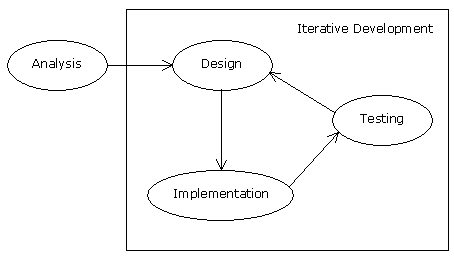
\includegraphics{images/ResearchMethodology}
	\caption{Overview of the research methodology}
	\label{fig:ResearchMethodology2}
\end{figure}

\subsection{Analysis}

In the analysis phase, the most widely used metamodelling architectures that enable engineers to define modelling languages and models, and the the most common model management tasks were identified. For each model management task, the state-of-the-art approaches in terms of supporting languages and tools were reviewed in order to identify their advantages and shortcomings. Through the analysis, a number of research challenges have been identified that have motivated the hypothesis and objectives of the thesis.

\subsection{Iterative Design and Implementation}

Following the analysis phase, a conceptual architecture has been conceived to investigate the hypothesis. This conceptual architecture has been refined into a technical design which in turn has guided the construction of a reference implementation.
 
In the first phase of design, infrastructure was designed based on the findings of the analysis. Following this, languages for previously unsupported tasks (model comparison and merging) were built atop the infrastructure. Through the process of building these first task-specific languages, the design and implementation of the infrastructure have been progressively improved and become more flexible in order to accommodate the needs of the different tasks. Latterly, languages for model-to-model transformation, model validation and in-place model transformation were designed and implemented. 

Finally, a workflow mechanism was designed and a prototype was implemented to enable orchestration and coordination of tasks implemented using different task-specific language of the platform.

\subsection{Iterative Testing}

Throughout the design and implementation iterations, several case studies have been used to assess the quality and usefulness of the proposed approach and the correctness of the reference implementation. Also significant feedback has been provided by the academic peers who have reviewed a number of publications on several core aspects of the design of the platform and the languages that built atop it, and by external users who have been using the reference implementation. Errors and omissions identified during testing iterations were provided as input to further design and implementation cycles.

\section{Chapter Summary}

This chapter has provided a detailed discussion on the research challenges identified during the background review performed in Chapter \ref{chp:LiteratureReview} and established the hypothesis and objectives of the thesis. The following chapters discuss the establishment and development of a platform of integrated languages for model management that is used as a means for exploring the proposed hypothesis.